%% 由 build/emit_tex.py 生成（生成物，勿手改）；定制请放 user_style.tex / user_meta.yaml
\chapter{第 3 章 ·
复变函数的积分}\label{ux7b2c-3-ux7ae0-ux590dux53d8ux51fdux6570ux7684ux79efux5206}

\section{3.1
复变函数积分的概念}\label{ux590dux53d8ux51fdux6570ux79efux5206ux7684ux6982ux5ff5}

\begin{quote}
本节目标：理解有向曲线的正向与负向约定，掌握复变函数积分的定义与四个基本性质，会用参数方程法（以及化归为两个实第二类曲线积分）计算复变函数积分。
重点：复变函数积分的定义、性质 3.1--3.4、定理 3.1 与参数方程法、典型积分
\(\int_C z^2dz\)、\(\int_C\operatorname{Im}(z)dz\)、\(\oint_C d z/(z-z_0)^{n+1}\)。
难点：积分的存在性定义（极限与分法、取点无关）；积分不等式 \(ML\)
估计；非解析函数积分与路径有关。
\end{quote}

\subsection{3.1.1
有向曲线与复变函数积分的定义}\label{ux6709ux5411ux66f2ux7ebfux4e0eux590dux53d8ux51fdux6570ux79efux5206ux7684ux5b9aux4e49}

设平面上光滑或分段光滑曲线 \(C\) 的两个端点为 \(A\) 和 \(B\)。\(C\)
可能有两个方向：从点 \(A\) 到点 \(B\) 和从点 \(B\) 到点
\(A\)。若规定其中一个方向（例如从点 \(A\) 到点 \(B\)
的方向）为正方向，则称 \(C\) 为\textbf{有向曲线}。此时称点 \(A\) 为曲线
\(C\) 的\textbf{起点}，点 \(B\) 为曲线 \(C\)
的\textbf{终点}。若正方向指从起点到终点的方向，那么从终点 \(B\) 到起点
\(A\) 的方向则称为曲线 \(C\) 的\textbf{负方向}，记作 \(C^-\)。

\textbf{定义 3.1} 设 \(C\) 为一条光滑或分段光滑的有向曲线，其中 \(A\)
为起点，\(B\) 为终点，函数 \(f(z)\) 在曲线 \(C\) 上有定义。现沿着 \(C\)
按从点 \(A\) 到点 \(B\) 的方向，在 \(C\) 上依次任取分点

\[
A=z_0,z_1,\dots,z_{n-1},z_n=B,
\]

将曲线 \(C\) 划分成 \(n\) 个小弧段 \(z_{k-1}z_k\)。在每个小弧段
\(z_{k-1}z_k\)（\(k=1,2,\dots,n\)）上任取一点 \(\zeta_k\)，并作和式

\[
S_n=\sum_{k=1}^{n}f(\zeta_k)\Delta z_k,\qquad \Delta z_k=z_k-z_{k-1}.
\]

记 \(\lambda\) 为 \(n\) 个小弧段长度中的最大值。当 \(\lambda\)
趋向于零时，若不论对曲线 \(C\) 的分法及点 \(\zeta_k\)
的取法如何，\(S_n\) 的极限存在，则称函数 \(f(z)\) 沿曲线 \(C\)
\textbf{可积}，并称这个极限值为函数 \(f(z)\) 沿曲线 \(C\) 的积分，记作

\[
\int_C f(z)\,dz=\lim_{\lambda\to 0}\sum_{k=1}^{n}f(\zeta_k)\Delta z_k .
\]

\(f(z)\) 称为\textbf{被积函数}，\(f(z)\,dz\) 称为\textbf{被积表达式}。

\begin{figure}
\centering
\pandocbounded{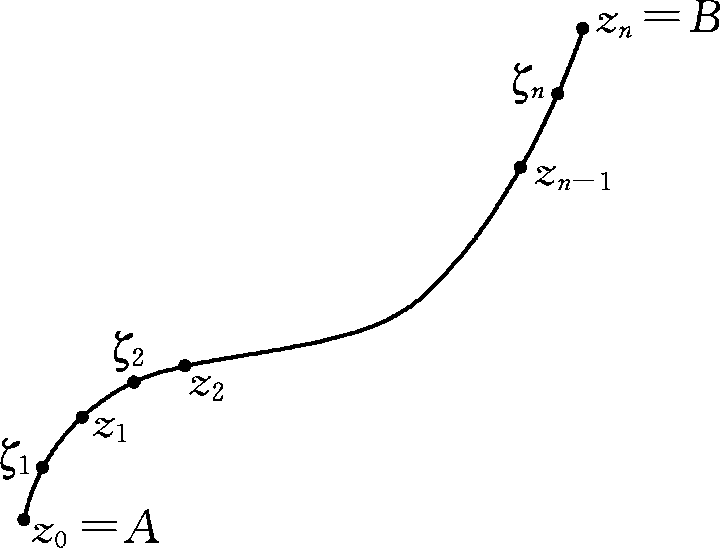
\includegraphics[keepaspectratio,alt={图3.1 曲线 C 的划分与积分和 S\_n}]{figures/03-复变函数的积分/fig-p03-6054f883.png}}
\caption{图3.1 曲线 \(C\) 的划分与积分和 \(S_n\)}
\end{figure}

\subsection{3.1.2
闭曲线上的积分与正方向}\label{ux95edux66f2ux7ebfux4e0aux7684ux79efux5206ux4e0eux6b63ux65b9ux5411}

若 \(C\) 为闭曲线，\(C\) 的正方向指的是：当点沿着曲线 \(C\)
按所选定取积分的方向运动时，\(C\) 所围区域始终在它的左侧。这时函数
\(f(z)\) 沿曲线 \(C\) 的积分记作

\[
\oint_C f(z)\,dz .
\]

\subsection{3.1.3
复变函数积分的性质}\label{ux590dux53d8ux51fdux6570ux79efux5206ux7684ux6027ux8d28}

\textbf{性质 3.1（方向性）} 若函数 \(f(z)\) 沿曲线 \(C\) 可积，则

\[
\int_C f(z)\,dz=-\int_{C^-} f(z)\,dz .
\]

\textbf{性质 3.2（线性性）} 若函数 \(f(z)\) 和 \(g(z)\) 沿曲线 \(C\)
可积，则

\[
\int_C\big[\alpha f(z)+\beta g(z)\big]\,dz
=\alpha\int_C f(z)\,dz+\beta\int_C g(z)\,dz,
\]

其中 \(\alpha,\beta\) 为任意常数。

\textbf{性质 3.3（对积分路径的可加性）} 若函数 \(f(z)\) 沿曲线 \(C\)
可积，曲线 \(C\) 由曲线段 \(C_1,C_2,\dots,C_n\) 依次首尾相接而成，则

\[
\int_C f(z)\,dz=\int_{C_1}f(z)\,dz+\int_{C_2}f(z)\,dz+\cdots+\int_{C_n}f(z)\,dz .
\]

\textbf{性质 3.4（积分不等式）} 若函数 \(f(z)\) 沿曲线 \(C\) 可积，且对
\(\forall z\in C\) 满足 \(|f(z)|\le M\)，曲线 \(C\) 的长度为 \(L\)，则

\[
\left|\int_C f(z)\,dz\right|\le\int_C |f(z)|\,ds\le ML,
\]

其中 \(ds=|dz|=\sqrt{dx^2+dy^2}\) 为曲线 \(C\) 的\textbf{弧微分}。

\textbf{证明要点} 记 \(\Delta s_k\) 为 \(z_{k-1}\) 与 \(z_k\)
之间的弧长，则

\[
\left|\sum_{k=1}^{n}f(\zeta_k)\Delta z_k\right|
\le\sum_{k=1}^{n}|f(\zeta_k)|\,|\Delta z_k|
\le\sum_{k=1}^{n}|f(\zeta_k)|\,\Delta s_k .
\]

令 \(\lambda\to 0\)，两端取极限得

\[
\left|\int_C f(z)\,dz\right|\le\int_C |f(z)|\,ds .
\]

又

\[
\sum_{k=1}^{n}|f(\zeta_k)|\,\Delta s_k\le M\sum_{k=1}^{n}\Delta s_k=ML,
\]

故

\[
\left|\int_C f(z)\,dz\right|\le\int_C |f(z)|\,ds\le ML .
\]

\subsection{3.1.4
复变函数积分的基本计算方法}\label{ux590dux53d8ux51fdux6570ux79efux5206ux7684ux57faux672cux8ba1ux7b97ux65b9ux6cd5}

\textbf{定理 3.1} 若函数 \(f(z)=u(x,y)+iv(x,y)\) 沿曲线 \(C\) 连续，则
\(f(z)\) 沿 \(C\) 可积，且

\[
\int_C f(z)\,dz=\int_C u\,dx-v\,dy+i\int_C v\,dx+u\,dy .
\]

\textbf{证明要点} 记 \(z_k=x_k+iy_k\)，\(\zeta_k=\xi_k+i\eta_k\)，则

\[
\Delta x_k=x_k-x_{k-1},\qquad \Delta y_k=y_k-y_{k-1},\qquad \Delta z_k=\Delta x_k+i\Delta y_k .
\]

于是

\[
\begin{aligned}
\sum_{k=1}^{n}f(\zeta_k)\Delta z_k
&=\sum_{k=1}^{n}\bigl(u(\xi_k,\eta_k)+iv(\xi_k,\eta_k)\bigr)(\Delta x_k+i\Delta y_k)\\
&=\sum_{k=1}^{n}\bigl[u(\xi_k,\eta_k)\Delta x_k-v(\xi_k,\eta_k)\Delta y_k\bigr]
+i\sum_{k=1}^{n}\bigl[v(\xi_k,\eta_k)\Delta x_k+u(\xi_k,\eta_k)\Delta y_k\bigr].
\end{aligned}
\]

已知 \(f(z)\) 沿 \(C\) 连续，所以必有 \(u,v\) 都沿 \(C\)
连续，于是这两个第二类曲线积分都存在，因此积分存在，且

\[
\int_C f(z)\,dz=\int_C u\,dx-v\,dy+i\int_C v\,dx+u\,dy .
\]

\textbf{参数方程法} 设 \(C\) 为一光滑或分段光滑曲线，其参数方程为

\[
z=z(t)=x(t)+iy(t)\quad(a\le t\le b),
\]

参数 \(t=a\) 时对应曲线 \(C\) 的起点，\(t=b\) 时对应曲线 \(C\) 的终点。

设 \(f(z)\) 沿曲线 \(C\) 连续，则

\[
f\bigl(z(t)\bigr)=u\bigl(x(t),y(t)\bigr)+iv\bigl(x(t),y(t)\bigr)=u(t)+iv(t),
\]

且

\[
\int_C f(z)\,dz=\int_a^b f\bigl(z(t)\bigr)z'(t)\,dt .
\]

其中

\[
\operatorname{Re}\bigl(f(z(t))z'(t)\bigr)=u(t)x'(t)-v(t)y'(t),
\]

\[
\operatorname{Im}\bigl(f(z(t))z'(t)\bigr)=u(t)y'(t)+v(t)x'(t).
\]

\subsection{3.1.5 典型例题}\label{ux5178ux578bux4f8bux9898}

\textbf{例 3.1} 分别沿下列路径计算积分 \(\int_C z^2\,dz\) 和
\(\int_C\operatorname{Im}(z)\,dz\)：

\begin{enumerate}
\def\labelenumi{\arabic{enumi}.}
\tightlist
\item
  \(C\) 为从原点 \((0,0)\) 到 \((1,1)\) 的直线段；
\item
  \(C\) 为从原点 \((0,0)\) 到 \((1,0)\) 再到 \((1,1)\) 的直线段。
\end{enumerate}

\textbf{解} (1) \(C\) 的参数方程为 \(z=(1+i)t\)，\(t\) 从 \(0\) 到
\(1\)，于是

\[
\int_C z^2\,dz
=\int_0^1\bigl[(1+i)t\bigr]^2 d\bigl((1+i)t\bigr)
=\int_0^1 (1+i)\bigl((1+i)t\bigr)^2dt
=(1+i)^3\int_0^1 t^2dt
=\frac{(1+i)^3}{3}.
\]

同时

\[
\int_C\operatorname{Im}(z)\,dz=\int_0^1 t\,d\bigl((1+i)t\bigr)=(1+i)\int_0^1 t\,dt=\frac{1+i}{2}.
\]

\begin{enumerate}
\def\labelenumi{(\arabic{enumi})}
\setcounter{enumi}{1}
\tightlist
\item
  把从 \((0,0)\) 到 \((1,0)\) 和从 \((1,0)\) 到 \((1,1)\)
  的两直线段分别记为 \(C_1\) 和 \(C_2\)。\(C_1\) 的参数方程为
  \(y=0\)，\(x\) 从 \(0\) 到 \(1\)；\(C_2\) 的参数方程为 \(x=1\)，\(y\)
  从 \(0\) 到 \(1\)。于是
\end{enumerate}

\[
\begin{aligned}
\int_C z^2\,dz
&=\int_{C_1}z^2\,dz+\int_{C_2}z^2\,dz
=\int_0^1 x^2\,dx+\int_0^1(1+iy)^2\,d(1+iy)\\
&=\frac{x^3}{3}\Big|_0^1+i\left(y-\frac{y^3}{3}+iy^2\right)\Big|_0^1
=\frac13+i-\frac{i}{3}-1=\frac{2i-2}{3}=\frac{(1+i)^3}{3},
\end{aligned}
\]

且

\[
\int_C\operatorname{Im}(z)\,dz=\int_0^1 0\,dx+\int_0^1 y\,d(1+iy)=\frac{i}{2}.
\]

\begin{quote}
说明：\(\int_C z^2dz\) 沿两条路径的值相同（因为 \(z^2\)
在复平面解析，积分与路径无关），而 \(\int_C\operatorname{Im}(z)dz\)
沿两条路径的值不同，说明非解析函数的积分一般与路径有关。
\end{quote}

\textbf{例 3.2} 计算积分 \(\oint_C \dfrac{\bar z}{z}\,dz\)，其中 \(C\)
为图 3.2 所示半圆环区域的正向边界。

\begin{figure}
\centering
\pandocbounded{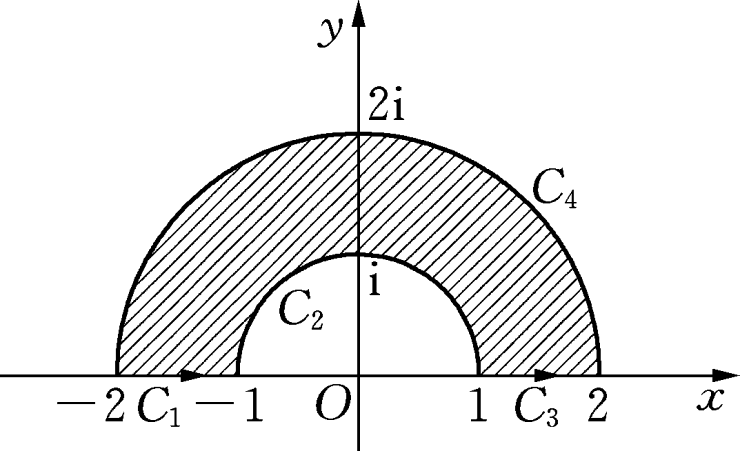
\includegraphics[keepaspectratio,alt={图3.2 半圆环区域及其正向边界}]{figures/03-复变函数的积分/fig-p12-3b3622a3.png}}
\caption{图3.2 半圆环区域及其正向边界}
\end{figure}

\textbf{解}
积分路径可分为四段：\(C_1:z=t\ (-2\le t\le -1)\)；\(C_2:z=e^{i\theta}\)（\(\theta\)
从 \(\pi\) 到
\(0\)）；\(C_3:z=t\ (1\le t\le 2)\)；\(C_4:z=2e^{i\theta}\)（\(\theta\)
从 \(0\) 到 \(\pi\)）。于是

\[
\begin{aligned}
\oint_C\frac{\bar z}{z}\,dz
&=\int_{C_1}\frac{\bar z}{z}\,dz+\int_{C_2}\frac{\bar z}{z}\,dz+\int_{C_3}\frac{\bar z}{z}\,dz+\int_{C_4}\frac{\bar z}{z}\,dz\\
&=\int_{-2}^{-1}\frac{t}{t}\,dt+\int_{\pi}^{0}\frac{e^{i\theta}}{e^{-i\theta}}\,i e^{i\theta}\,d\theta
+\int_{1}^{2}\frac{t}{t}\,dt+\int_{0}^{\pi}\frac{2e^{i\theta}}{2e^{-i\theta}}\,2i e^{i\theta}\,d\theta\\
&=1+\frac23+1-\frac43=\frac43 .
\end{aligned}
\]

\begin{quote}
注：幻灯片对两条圆弧的代入写作
\(\dfrac{e^{i\theta}}{e^{-i\theta}}\)，这对应的是
\(\dfrac{z}{\bar z}\)；若严格按题面 \(\dfrac{\bar z}{z}\)
计算，两条圆弧分别得 \(-2\) 与 \(4\)，总值为
\(4\)。此处按幻灯片原式与结果 \(4/3\) 转写，请以教材/课堂为准。
\end{quote}

\textbf{例 3.3} 计算积分 \(\oint_C\dfrac{dz}{(z-z_0)^{n+1}}\)，其中
\(C\) 为以 \(z_0\) 为中心、\(r\) 为半径的正向圆周，\(n\) 为整数。

\textbf{解} 曲线 \(C\) 的方程为
\(z=z_0+re^{i\theta}\ (0\le\theta\le2\pi)\)，于是

\[
I=\oint_C\frac{dz}{(z-z_0)^{n+1}}
=\int_0^{2\pi}\frac{i r e^{i\theta}d\theta}{r^{n+1}e^{i(n+1)\theta}}
=\int_0^{2\pi}\frac{i}{r^n e^{in\theta}}d\theta
=\frac{i}{r^n}\int_0^{2\pi}e^{-in\theta}d\theta .
\]

当 \(n=0\) 时，

\[
I=i\int_0^{2\pi}d\theta=2\pi i ;
\]

当 \(n\neq0\) 时，

\[
I=\frac{i}{r^n}\int_0^{2\pi}(\cos n\theta-i\sin n\theta)\,d\theta=0 .
\]

因此

\[
\oint_{|z-z_0|=r}\frac{dz}{(z-z_0)^{n+1}}
=\begin{cases}2\pi i, & n=0,\\ 0, & n\neq0.\end{cases}
\]

\begin{figure}
\centering
\pandocbounded{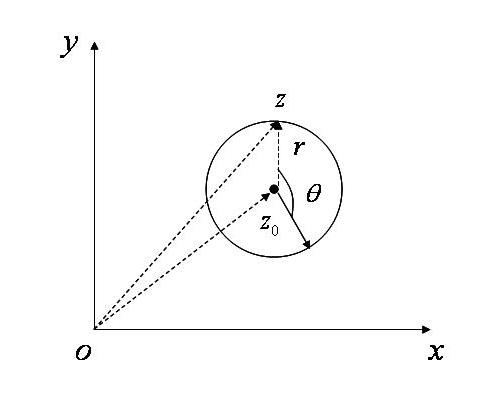
\includegraphics[keepaspectratio,alt={图3.3 以 z\_0 为圆心的正向圆周}]{figures/03-复变函数的积分/fig-p13-8809ed0a.jpg}}
\caption{图3.3 以 \(z_0\) 为圆心的正向圆周}
\end{figure}

\subsection{常见错误与注意点}\label{ux5e38ux89c1ux9519ux8befux4e0eux6ce8ux610fux70b9-7}

\begin{enumerate}
\def\labelenumi{\arabic{enumi}.}
\tightlist
\item
  \textbf{方向约定}：\(\int_C=-\int_{C^-}\)；闭曲线的正向是使其所围区域始终位于左侧的方向（通常取逆时针）。
\item
  \textbf{积分不等式}：左端是``积分模''的不等式，右端用弧长作估计，\(ds=|dz|\)，最终有
  \(ML\)；不要遗漏``总长度 \(L\)''这一因子。
\item
  \textbf{\(\operatorname{Im}(z)\) 的积分}：\(\operatorname{Im}(z)\)
  不是解析函数，其积分一般与路径有关，不能像解析函数那样随意换路径。
\item
  \textbf{例 3.2 的记号}：幻灯片解法的圆弧代入写的是
  \(\dfrac{z}{\bar z}\)（即
  \(\dfrac{e^{i\theta}}{e^{-i\theta}}\)），与题面 \(\dfrac{\bar z}{z}\)
  不一致，注意区分两者的积分值。
\end{enumerate}

\subsection{本节小结}\label{ux672cux8282ux5c0fux7ed3-7}

\begin{itemize}
\tightlist
\item
  \textbf{定义}：\(\int_C f(z)dz=\lim\limits_{\lambda\to0}\sum_{k}f(\zeta_k)\Delta z_k\)，其中
  \(\Delta z_k=z_k-z_{k-1}\)。
\item
  \textbf{性质}：方向性、线性性、路径可加性、积分不等式（\(ML\) 估计）。
\item
  \textbf{计算方法}：化归为两个第二类曲线积分，或参数方程法
  \(\int_C f(z)dz=\int_a^b f(z(t))z'(t)dt\)。
\item
  \textbf{重要结果}：\(\oint_{|z-z_0|=r}\dfrac{dz}{(z-z_0)^{n+1}}=\begin{cases}2\pi i,& n=0,\\0,& n\ne0.\end{cases}\)
\end{itemize}

\section{3.2
柯西-古萨定理及其推广}\label{ux67efux897f-ux53e4ux8428ux5b9aux7406ux53caux5176ux63a8ux5e7f}

\begin{quote}
本节目标：理解并掌握柯西-古萨定理及其推论，理解单连通域内``积分与路径无关''的本质，掌握原函数、变上限函数与牛顿-莱布尼茨型公式，并能运用复合闭路定理处理多连通区域上有奇点时的积分。
重点：柯西-古萨定理（\(\oint_C f(z)dz=0\)）、推论 3.1/3.2、原函数与定理
3.3/3.4、复合闭路定理（定理 3.5）及应用。
难点：格林公式与柯西-黎曼方程在证明中的作用；多连通区域与复闭路；奇点与复合闭路选取。
\end{quote}

\subsection{3.2.1
柯西-古萨（Cauchy-Goursat）定理}\label{ux67efux897f-ux53e4ux8428cauchy-goursatux5b9aux7406}

假设函数 \(f(z)=u+iv\) 在单连通域 \(D\) 内处处解析，\(f'(z)\) 在 \(D\)
内连续，\(u,v\) 对 \(x,y\) 的偏导数在 \(D\) 内连续。设 \(z=x+iy\)，\(C\)
为 \(D\) 内任一条简单闭曲线。由定理 3.1 有

\[
\int_C f(z)\,dz=\int_C u\,dx-v\,dy+i\int_C v\,dx+u\,dy .
\]

记 \(G\) 为 \(C\) 所围区域，由格林（Green）公式有

\[
\int_C u\,dx-v\,dy=\iint_G\left(-\frac{\partial v}{\partial x}-\frac{\partial u}{\partial y}\right)dxdy .
\]

由于 \(f(z)=u+iv\) 在 \(D\) 内解析，所以 \(u,v\) 在 \(D\)
内处处满足柯西-黎曼方程，即

\[
\frac{\partial u}{\partial x}=\frac{\partial v}{\partial y},\qquad \frac{\partial v}{\partial x}=-\frac{\partial u}{\partial y}.
\]

因此

\[
\int_C u\,dx-v\,dy=\int_C v\,dx-u\,dy=0,
\]

从而

\[
\oint_C f(z)\,dz=0 .
\]

\textbf{定理 3.2（柯西-古萨定理）} 若函数 \(f(z)\) 是单连通域 \(D\)
内的解析函数，则 \(f(z)\) 沿 \(D\) 内任一条闭曲线 \(C\) 的积分为零，即

\[
\oint_C f(z)\,dz=0 .
\]

任意一条闭曲线都可以看成是由有限多条简单闭曲线衔接而成的。

\begin{figure}
\centering
\pandocbounded{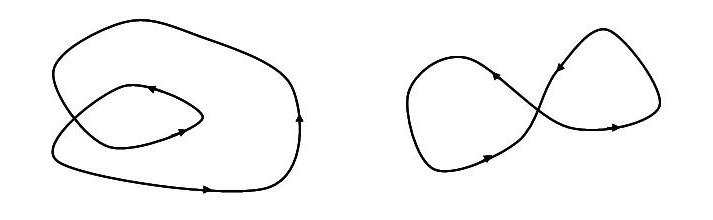
\includegraphics[keepaspectratio,alt={图3.4 闭曲线分解为有限多条简单闭曲线}]{figures/03-复变函数的积分/fig-p15-c94f538e.jpg}}
\caption{图3.4 闭曲线分解为有限多条简单闭曲线}
\end{figure}

\subsection{3.2.2
柯西-古萨定理的推论}\label{ux67efux897f-ux53e4ux8428ux5b9aux7406ux7684ux63a8ux8bba}

\textbf{推论 3.1} 设 \(C\) 为 \(z\) 平面上的一条闭曲线，它围成单连通域
\(D\)，若函数 \(f(z)\) 在 \(\bar D=D\cup C\) 上解析，则

\[
\oint_C f(z)\,dz=0 .
\]

\textbf{推论 3.2} 设函数 \(f(z)\) 在单连通域 \(D\) 解析，则 \(f(z)\) 在
\(D\) 内积分与路径无关。即积分 \(\int_C f(z)dz\) 不依赖于连接起点
\(z_0\) 与终点 \(z_1\) 的曲线 \(C\)，而只与 \(z_0\)、\(z_1\)
的位置有关。

\textbf{证明要点} 设 \(C_1\) 和 \(C_2\) 为 \(D\) 内连接 \(z_0\) 与
\(z_1\) 的任意两条曲线。显然 \(C_1\) 与 \(C_2^-\) 连接成 \(D\)
内一条闭曲线 \(C\)。由柯西-古萨定理

\[
\int_{C_1}f(z)\,dz+\int_{C_2^-}f(z)\,dz=\oint_C f(z)\,dz=0 .
\]

故

\[
\int_{C_1}f(z)\,dz=\int_{C_2}f(z)\,dz .
\]

\begin{figure}
\centering
\pandocbounded{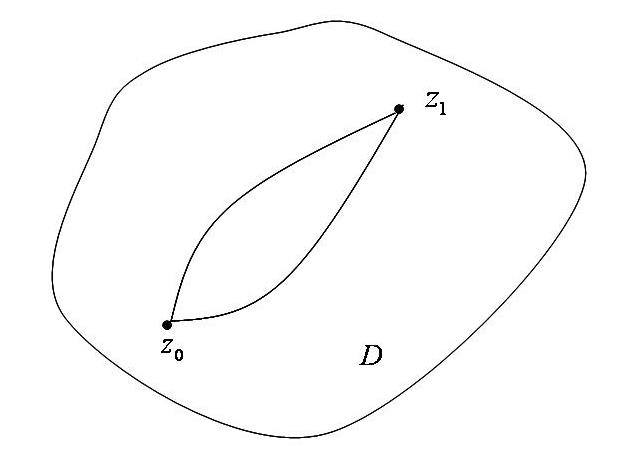
\includegraphics[keepaspectratio,alt={图3.5 积分与路径无关}]{figures/03-复变函数的积分/fig-p16-23ad9722.jpg}}
\caption{图3.5 积分与路径无关}
\end{figure}

\subsection{3.2.3 原函数}\label{ux539fux51fdux6570}

函数 \(f(z)\) 沿曲线 \(C_1\) 和 \(C_2\) 的积分又可以表示为

\[
\int_{C_1}f(z)\,dz=\int_{C_2}f(z)\,dz=\int_{z_0}^{z_1}f(z)\,dz .
\]

固定下限 \(z_0\)，让上限 \(z_1\) 在区域 \(D\) 内变动，并令
\(z_1=z\)，则确定了一个关于上限 \(z\) 的单值函数

\[
F(z)=\int_{z_0}^{z}f(\zeta)\,d\zeta .
\]

并称 \(F(z)\) 为定义在区域 \(D\)
内的\textbf{积分上限函数}或\textbf{变上限函数}。

\textbf{定理 3.3} 若函数 \(f(z)\) 在单连通域 \(D\) 内解析，则函数
\(F(z)\) 必在 \(D\) 内解析，且 \(F'(z)=f(z)\)。

\textbf{证明要点} 若 \(D\) 内任取一点 \(z\)，以 \(z\) 为中心作一个含于
\(D\) 内的小圆 \(B\)，在 \(B\) 内取点
\(z+\Delta z\)（\(\Delta z\neq0\)）。由积分与路径无关，

\[
F(z+\Delta z)-F(z)=\int_{z_0}^{z+\Delta z}f(\zeta)\,d\zeta-\int_{z_0}^{z}f(\zeta)\,d\zeta=\int_{z}^{z+\Delta z}f(\zeta)\,d\zeta .
\]

而 \(f(z)\) 是与积分变量 \(\zeta\) 无关的值，故

\[
\int_{z}^{z+\Delta z}f(z)\,d\zeta=f(z)\int_{z}^{z+\Delta z}d\zeta=f(z)\Delta z .
\]

于是

\[
\frac{F(z+\Delta z)-F(z)}{\Delta z}-f(z)
=\frac{1}{\Delta z}\int_{z}^{z+\Delta z}\bigl(f(\zeta)-f(z)\bigr)d\zeta .
\]

又 \(f(z)\) 在 \(D\) 内解析，显然 \(f(z)\) 在 \(D\)
内连续。所以对于任给的 \(\varepsilon>0\)，必存在 \(\delta>0\)，使得当
\(|\zeta-z|<\delta\)（且 \(\zeta\) 落在圆 \(B\) 内），即当
\(|\Delta z|<\delta\) 时，总有 \(|f(\zeta)-f(z)|<\varepsilon\)，从而

\[
\left|\frac{F(z+\Delta z)-F(z)}{\Delta z}-f(z)\right|
\le\frac{1}{|\Delta z|}\int_{z}^{z+\Delta z}|f(\zeta)-f(z)|\,d\zeta
\le\frac{1}{|\Delta z|}\varepsilon|\Delta z|=\varepsilon .
\]

故

\[
\lim_{\Delta z\to0}\frac{F(z+\Delta z)-F(z)}{\Delta z}=f(z),\qquad F'(z)=f(z) .
\]

\begin{figure}
\centering
\pandocbounded{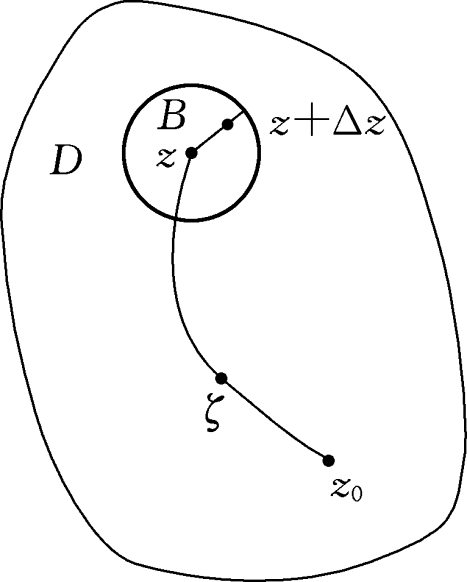
\includegraphics[keepaspectratio,alt={图3.6 定理3.3证明中的小圆 B}]{figures/03-复变函数的积分/fig-p18-e9084205.png}}
\caption{图3.6 定理3.3证明中的小圆 \(B\)}
\end{figure}

\textbf{定义 3.2} 若在区域 \(D\) 内，\(\varphi(z)\) 的导数等于
\(f(z)\)，则称 \(\varphi(z)\) 为 \(f(z)\) 在 \(D\)
内的\textbf{原函数}。变上限函数

\[
F(z)=\int_{z_0}^{z}f(\zeta)\,d\zeta
\]

为 \(f(z)\) 的一个原函数。那么函数 \(f(z)\) 的全体原函数可以表示为

\[
\varphi(z)=F(z)+C,
\]

其中 \(C\) 为任意常数。

\textbf{定理 3.4} 若函数 \(f(z)\) 在单连通域 \(D\)
内处处解析，\(\varphi(z)\) 为 \(f(z)\) 的一个原函数，则

\[
\int_{z_0}^{z_1}f(z)\,dz=\varphi(z_1)-\varphi(z_0)=\varphi(z)\Big|_{z_0}^{z_1},
\]

其中 \(z_0\)、\(z_1\) 为 \(D\) 内的点。

\textbf{证明要点} \(F(z)=\int_{z_0}^{z}f(\zeta)\,d\zeta\) 为 \(f(z)\)
的一个原函数，故

\[
F(z)=\int_{z_0}^{z}f(\zeta)\,d\zeta=\varphi(z)+C .
\]

当 \(z=z_0\) 时，根据柯西-古萨定理可知

\[
\int_{z_0}^{z_0}f(\zeta)\,d\zeta=\varphi(z_0)-\varphi(z_0)=0 .
\]

于是 \(C=-\varphi(z_0)\)，故

\[
\int_{z_0}^{z_1}f(z)\,dz=\varphi(z_1)-\varphi(z_0) .
\]

\textbf{例 3.4} 求积分 \(\displaystyle\int_0^{\pi i/2}\sin 2z\,dz\)
的值。

\textbf{解} 因为 \(\sin 2z\) 在复平面上解析，所以积分与路径无关。

\[
\int_0^{\pi i/2}\sin 2z\,dz
=-\frac12\cos 2z\Big|_0^{\pi i/2}
=-\frac12(\cos\pi i-\cos0)
=-\frac12\left(\frac{e^{-\pi}+e^{\pi}}{2}-1\right)
=\frac12-\frac{e^{-\pi}+e^{\pi}}{4}.
\]

\textbf{例 3.5} 求积分 \(\displaystyle\int_0^i(z-1)e^{-z}\,dz\) 的值。

\textbf{解} 因为 \((z-1)e^{-z}\) 在复平面上解析，所以积分与路径无关。

\[
\int_0^i(z-1)e^{-z}\,dz=\int_0^i ze^{-z}\,dz-\int_0^i e^{-z}\,dz .
\]

上式右边第一个积分采用分部积分法，第二个积分可用凑微分法：

\[
\int_0^i(z-1)e^{-z}\,dz
=-ze^{-z}\Big|_0^i+\int_0^i e^{-z}\,dz-\int_0^i e^{-z}\,dz
=-ie^{-i}=-\sin1-i\cos1 .
\]

\subsection{3.2.4
复合闭路定理}\label{ux590dux5408ux95edux8defux5b9aux7406}

设有 \(n+1\) 条简单闭曲线 \(C_0,C_1,C_2,\dots,C_n\)，其中
\(C_1,C_2,\dots,C_n\) 互不相交也互不包含，并且都含于 \(C_0\) 的内部。这
\(n+1\) 条曲线围成了一个多连通区域 \(D\)，\(D\) 的边界 \(C\)
称作\textbf{复闭路}，它的正向为 \(C_0\)
取逆时针方向，其它曲线都取顺时针方向。因此复闭路记作

\[
C=C_0+C_1^-+C_2^-+\cdots+C_n^- .
\]

\textbf{定理 3.5} 若 \(f(z)\) 在复闭路
\(C=C_0+C_1^-+C_2^-+\cdots+C_n^-\) 及其所围成的多连通区域内解析，则

\[
\oint_{C_0}f(z)\,dz=\oint_{C_1}f(z)\,dz+\oint_{C_2}f(z)\,dz+\cdots+\oint_{C_n}f(z)\,dz ,
\]

也就是

\[
\oint_C f(z)\,dz=0 .
\]

\textbf{证明要点} 做辅助线 \(l_1,l_2,l_3\) 将 \(C_0\)、\(C_1\) 及
\(C_2\) 连接起来，从而把多连通区域 \(D\) 划分为两个单连通区域 \(D_1\) 及
\(D_2\)，并分别用 \(\Gamma_1\) 及 \(\Gamma_2\)
表示这两个区域的边界。由柯西-古萨定理

\[
\oint_{\Gamma_1}f(z)\,dz=0,\qquad \oint_{\Gamma_2}f(z)\,dz=0 .
\]

两式相加，辅助线上的积分正负相抵，得

\[
\oint_{C_0}f(z)\,dz-\oint_{C_1}f(z)\,dz-\oint_{C_2}f(z)\,dz=0,
\]

故

\[
\oint_{C_0}f(z)\,dz=\oint_{C_1}f(z)\,dz+\oint_{C_2}f(z)\,dz .
\]

\begin{figure}
\centering
\pandocbounded{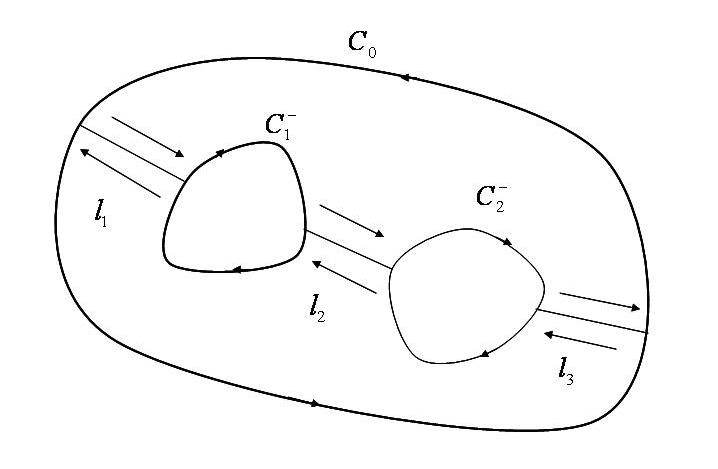
\includegraphics[keepaspectratio,alt={图3.7 复合闭路定理的证明}]{figures/03-复变函数的积分/fig-p25-f1470cb5.jpg}}
\caption{图3.7 复合闭路定理的证明}
\end{figure}

\textbf{例 3.6} 计算 \(\oint_C\dfrac{dz}{z^2+z}\) 的值，\(C\) 为包含圆周
\(|z|=1\) 在内的任何正向简单闭曲线。

\textbf{解} 显然 \(z=0\) 和 \(z=-1\) 是函数 \(\dfrac{1}{z^2+z}\)
的两个奇点。由于 \(C\) 为包含圆周 \(|z|=1\)
在内的任何正向简单闭曲线，因此也包含了这两个奇点。在 \(C\)
的内部作两个互不包含、互不相交的正向圆周 \(C_1\) 和 \(C_2\)，其中
\(C_1\) 的内部只包含奇点 \(z=-1\)，\(C_2\) 的内部只包含奇点
\(z=0\)。函数 \(\dfrac{1}{z^2+z}\) 在由 \(C\)、\(C_1\)、\(C_2\)
所围成的多连通域内解析，由复合闭路定理及例 3.3，

\[
\begin{aligned}
\oint_C\frac{dz}{z^2+z}
&=\oint_{C_1}\frac{dz}{z^2+z}+\oint_{C_2}\frac{dz}{z^2+z}\\
&=\oint_{C_1}\left(\frac{1}{z}-\frac{1}{z+1}\right)dz
+\oint_{C_2}\left(\frac{1}{z}-\frac{1}{z+1}\right)dz\\
&=0-2\pi i+2\pi i-0=0 .
\end{aligned}
\]

\subsection{常见错误与注意点}\label{ux5e38ux89c1ux9519ux8befux4e0eux6ce8ux610fux70b9-8}

\begin{enumerate}
\def\labelenumi{\arabic{enumi}.}
\tightlist
\item
  \textbf{单连通域是前提}：\(f(z)\) 必须是单连通域 \(D\)
  内的解析函数，才能保证
  \(\oint_C f(z)dz=0\)；若闭曲线内部有奇点，不能直接用柯西-古萨定理。
\item
  \textbf{方向}：复合闭路中外边界 \(C_0\) 取逆时针，内边界 \(C_i\)
  取顺时针；符号不能写反。
\item
  \textbf{原函数存在性}：只有在单连通域内解析的函数才处处有原函数；在非单连通域内变上限函数可能不解析（多值）。
\item
  \textbf{牛顿-莱布尼茨公式}：\(\int_{z_0}^{z_1}f(z)dz=\varphi(z_1)-\varphi(z_0)\)
  的前提是 \(f\) 在单连通域内解析且 \(\varphi\) 是其一原函数。
\item
  \textbf{例 3.6}：要先把 \(\dfrac{1}{z^2+z}\) 拆成
  \(\dfrac1z-\dfrac1{z+1}\)，再分别对每个奇点使用例 3.3 的结论。
\end{enumerate}

\subsection{本节小结}\label{ux672cux8282ux5c0fux7ed3-8}

\begin{itemize}
\tightlist
\item
  \textbf{柯西-古萨定理}：单连通域内解析函数沿闭曲线积分为零。
\item
  \textbf{推论}：\(f\) 在 \(\bar D=D\cup C\) 上解析
  \(\Rightarrow\oint_C fdz=0\)；单连通域内积分与路径无关。
\item
  \textbf{原函数}：变上限函数 \(F(z)=\int_{z_0}^z f(\zeta)d\zeta\)
  解析且 \(F'(z)=f(z)\)；一般原函数 \(\varphi(z)=F(z)+C\)。
\item
  \textbf{定理 3.4}：\(\int_{z_0}^{z_1}fdz=\varphi(z_1)-\varphi(z_0)\)。
\item
  \textbf{复合闭路定理}：多连通区域上
  \(\oint_{C_0}fdz=\sum\oint_{C_i}fdz\)（内边界取顺时针）。
\end{itemize}

\section{3.3
柯西积分公式及其推论}\label{ux67efux897fux79efux5206ux516cux5f0fux53caux5176ux63a8ux8bba}

\begin{quote}
本节目标：掌握柯西积分公式及其证明思想，理解解析函数的高阶导数公式与解析函数无穷次可导的性质，能灵活运用柯西积分公式与高阶导数公式计算闭路积分；了解平均值定理。
重点：柯西积分公式、高阶导数公式、定理
3.8/3.9，及其在计算闭路积分中的应用（例 3.7--3.10）。
难点：柯西积分公式的证明（复合闭路、\(r\to0\)
估计）；高阶导数公式中的``导数阶数''与``极点阶数''匹配；含多个奇点时的拆分。
\end{quote}

\subsection{3.3.1
柯西（Cauchy）积分公式}\label{ux67efux897fcauchyux79efux5206ux516cux5f0f}

\textbf{定理 3.6} 若 \(f(z)\) 是区域 \(D\) 内的解析函数，\(C\) 为 \(D\)
内的简单闭曲线，\(C\) 所围内部全含于 \(D\) 内，\(z\) 为 \(C\)
内部任一点，则

\[
f(z)=\frac{1}{2\pi i}\oint_C\frac{f(\zeta)}{\zeta-z}\,d\zeta,
\]

其中积分沿曲线 \(C\) 的正向。上式称为\textbf{柯西积分公式}。

\textbf{证明要点} 取定 \(C\) 内部一点 \(z\)。因为 \(f(z)\) 在 \(D\)
内解析，所以 \(f(z)\) 在点 \(z\) 连续，即对任给的
\(\forall\varepsilon>0\)，必存在 \(\delta>0\)，当 \(|\zeta-z|<\delta\)
时，有 \(|f(\zeta)-f(z)|<\varepsilon\)。

令

\[
F(\zeta)=\frac{f(\zeta)}{\zeta-z},
\]

则 \(F(\zeta)\) 在 \(D\) 内除去点 \(z\) 外处处解析。现以 \(z\)
为中心、\(r\) 为半径作圆周

\[
B:|\zeta-z|=r,
\]

使圆 \(B\) 的内部及边界全含于 \(C\) 的内部。由复合闭路定理有

\[
\oint_C\frac{f(\zeta)}{\zeta-z}\,d\zeta=\oint_B\frac{f(\zeta)}{\zeta-z}\,d\zeta .
\]

令 \(r\to0\)，只需证明

\[
\oint_B\frac{f(\zeta)}{\zeta-z}\,d\zeta\to2\pi i f(z) .
\]

因为

\[
\oint_B\frac{1}{\zeta-z}\,d\zeta=2\pi i ,
\]

而 \(f(z)\) 与 \(\zeta\) 无关，于是

\[
\begin{aligned}
\left|\oint_B\frac{f(\zeta)}{\zeta-z}\,d\zeta-2\pi i f(z)\right|
&=\left|\oint_B\frac{f(\zeta)-f(z)}{\zeta-z}\,d\zeta\right|\\
&\le\oint_B\frac{|f(\zeta)-f(z)|}{|\zeta-z|}\,|d\zeta|
\le\oint_B\frac{\varepsilon}{r}\,ds
=\frac{\varepsilon}{r}\cdot2\pi r=2\pi\varepsilon .
\end{aligned}
\]

当 \(r\to0\)（从而
\(\zeta\to z\)）时，\(2\pi\varepsilon\to0\)，故柯西积分公式成立。

\begin{figure}
\centering
\pandocbounded{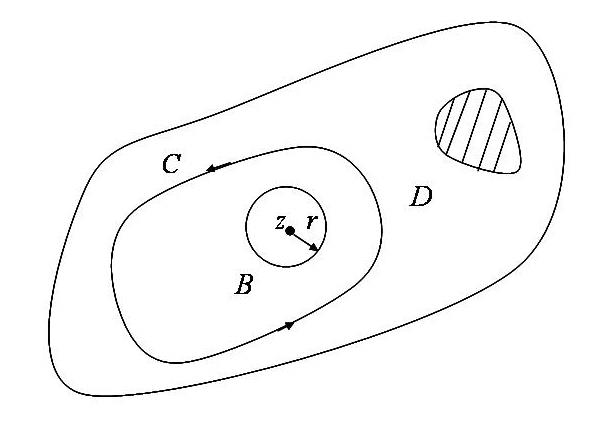
\includegraphics[keepaspectratio,alt={图3.8 柯西积分公式证明中的圆周 B}]{figures/03-复变函数的积分/fig-p28-7facc483.jpg}}
\caption{图3.8 柯西积分公式证明中的圆周 \(B\)}
\end{figure}

\textbf{平均值定理} 若函数 \(f(z)\) 在曲线 \(C\) 上恒为常数
\(K\)，\(z_0\) 为 \(C\) 内部任一点，则由柯西积分公式

\[
f(z)=\frac{1}{2\pi i}\oint_C\frac{f(\zeta)}{\zeta-z_0}\,d\zeta
=\frac{K}{2\pi i}\oint_C\frac{1}{\zeta-z_0}\,d\zeta
=\frac{K}{2\pi i}\cdot2\pi i=K,
\]

即 \(f(z)\) 在曲线 \(C\) 的内部也恒为常数 \(K\)。

若 \(C\) 为圆周 \(|\zeta-z_0|=R\)，即

\[
\zeta=z_0+Re^{i\theta}\quad(0\le\theta\le2\pi),
\]

则 \(d\zeta=iRe^{i\theta}d\theta\)，从而

\[
f(z_0)=\frac{1}{2\pi i}\oint_C\frac{f(\zeta)}{\zeta-z_0}\,d\zeta
=\frac{1}{2\pi}\int_0^{2\pi}f(z_0+Re^{i\theta})\,d\theta .
\]

\textbf{解析函数在圆心 \(z_0\)
处的值等于它在圆周上的平均值，这就是解析函数的平均值定理。}

若 \(f(z)\) 在简单闭曲线 \(C\) 所围成的区域内解析，且在 \(C\)
上连续，则柯西积分公式仍然成立。柯西积分公式可以改写成

\[
\oint_C\frac{f(\zeta)}{\zeta-z}\,d\zeta=2\pi i f(z) .
\]

\subsection{3.3.2
柯西积分公式的应用}\label{ux67efux897fux79efux5206ux516cux5f0fux7684ux5e94ux7528}

\textbf{例 3.7} 计算积分 \(\oint_{|z|=2}\dfrac{z^2+1}{z}\,dz\) 的值。

\textbf{解} 因为 \(z^2+1\) 在 \(|z|=2\) 内解析，

\[
\oint_{|z|=2}\frac{z^2+1}{z}\,dz
=2\pi i\cdot(z^2+1)\big|_{z=0}=2\pi i .
\]

\textbf{例 3.8} 计算积分
\(\oint_C\dfrac{\sin\frac{\pi z}{6}}{z^2-1}\,dz\) 的值，其中 \(C\) 为：

\begin{enumerate}
\def\labelenumi{\arabic{enumi}.}
\tightlist
\item
  \(|z-\frac32|=1\)；
\item
  \(|z+\frac32|=1\)；
\item
  \(|z|=3\)。
\end{enumerate}

\textbf{解} (1) 被积函数 \(\dfrac{\sin\frac{\pi z}{6}}{z+1}\) 在
\(|z-\frac32|=1\) 的内部解析，故

\[
\oint_C\frac{\sin\frac{\pi z}{6}}{z^2-1}\,dz
=\oint_C\frac{\sin\frac{\pi z}{6}}{z+1}\cdot\frac{1}{z-1}\,dz
=2\pi i\left(\frac{\sin\frac{\pi z}{6}}{z+1}\right)\Big|_{z=1}
=2\pi i\cdot\frac14=\frac{\pi i}{2}.
\]

\begin{enumerate}
\def\labelenumi{(\arabic{enumi})}
\setcounter{enumi}{1}
\tightlist
\item
  被积函数 \(\dfrac{\sin\frac{\pi z}{6}}{z-1}\) 在 \(|z+\frac32|=1\)
  的内部解析，故
\end{enumerate}

\[
\oint_C\frac{\sin\frac{\pi z}{6}}{z^2-1}\,dz
=\oint_C\frac{\sin\frac{\pi z}{6}}{z-1}\cdot\frac{1}{z+1}\,dz
=2\pi i\left(\frac{\sin\frac{\pi z}{6}}{z-1}\right)\Big|_{z=-1}
=2\pi i\cdot\frac14=\frac{\pi i}{2}.
\]

\begin{enumerate}
\def\labelenumi{(\arabic{enumi})}
\setcounter{enumi}{2}
\tightlist
\item
  被积函数在 \(|z|=3\) 的内部有两个奇点 \(z=1\) 和 \(z=-1\)。在 \(C\)
  的内部作两个互不包含、互不相交的正向圆周 \(C_1\) 和 \(C_2\)，其中
  \(C_1\) 的内部只包含奇点 \(z=1\)，\(C_2\) 的内部只包含奇点
  \(z=-1\)。由复合闭路定理及柯西积分公式，
\end{enumerate}

\[
\oint_C\frac{\sin\frac{\pi z}{6}}{z^2-1}\,dz
=\oint_{C_1}\frac{\sin\frac{\pi z}{6}}{z^2-1}\,dz+\oint_{C_2}\frac{\sin\frac{\pi z}{6}}{z^2-1}\,dz
=\frac{\pi i}{2}+\frac{\pi i}{2}=\pi i .
\]

\subsection{3.3.3
高阶导数公式}\label{ux9ad8ux9636ux5bfcux6570ux516cux5f0f}

\textbf{定理 3.7} 定义在区域 \(D\) 的解析函数 \(f(z)\) 有各阶导数，且有

\[
f^{(n)}(z)=\frac{n!}{2\pi i}\oint_C\frac{f(\zeta)}{(\zeta-z)^{n+1}}\,d\zeta\quad(n=1,2,\cdots),
\]

其中 \(C\) 为区域 \(D\) 内围绕 \(z\) 的任何一条简单闭曲线，积分沿曲线
\(C\) 的正向。

\textbf{定理 3.8} 若 \(f(z)\) 为定义在区域 \(D\) 内的解析函数，则在
\(D\)
内其各阶导数都存在并且解析。换句话说，\textbf{解析函数的导数也是解析函数}。

\textbf{定理 3.9} 函数 \(f(z)=u(x,y)+iv(x,y)\) 在区域 \(D\)
内解析的充要条件是：

\begin{enumerate}
\def\labelenumi{\arabic{enumi}.}
\tightlist
\item
  \(u_x,u_y,v_x,v_y\) 在 \(D\) 内连续；
\item
  \(u(x,y),v(x,y)\) 在 \(D\) 内满足柯西-黎曼方程
\end{enumerate}

\[
\frac{\partial u}{\partial x}=\frac{\partial v}{\partial y},\qquad \frac{\partial u}{\partial y}=-\frac{\partial v}{\partial x}.
\]

\textbf{例 3.9} 求积分
\(\oint_C\dfrac{e^z}{\left(z-\dfrac{\pi i}{2}\right)^2}\,dz\) 的值，其中
\(C\) 为 \(x^2+y^2=6y\)。

\textbf{解} 被积函数在 \(C\) 的内部有一个奇点
\(z=\dfrac{\pi i}{2}\)。由高阶导数公式（\(n=1\)），

\[
\oint_C\frac{e^z}{\left(z-\frac{\pi i}{2}\right)^2}\,dz
=2\pi i\left(e^z\right)'\Big|_{z=\pi i/2}
=2\pi i\,e^{\pi i/2}=2\pi i\cdot i=-2\pi .
\]

\textbf{例 3.10} 求积分 \(\oint_C\dfrac{\cos\pi z}{z^3(z-1)^2}\,dz\)
的值，其中 \(C\) 为 \(|z|=2\)。

\textbf{解} 被积函数在 \(C\) 的内部有两个奇点 \(z=0\) 和
\(z=1\)。作两条互不相交且互不包含的闭曲线 \(C_1\) 和
\(C_2\)，分别包围奇点 \(z=0\) 和 \(z=1\)，且两曲线所围区域全含于 \(C\)
的内部。由复合闭路定理和高阶导数公式，

\[
\begin{aligned}
\oint_C\frac{\cos\pi z}{z^3(z-1)^2}\,dz
&=\oint_{C_1}\frac{\cos\pi z}{(z-1)^2}\cdot\frac{1}{z^3}\,dz
+\oint_{C_2}\frac{\cos\pi z}{z^3}\cdot\frac{1}{(z-1)^2}\,dz\\
&=\frac{2\pi i}{2!}\left(\frac{\cos\pi z}{(z-1)^2}\right)''\Big|_{z=0}
+2\pi i\left(\frac{\cos\pi z}{z^3}\right)'\Big|_{z=1}\\
&=(6-\pi^2)\pi i+6\pi i=(12-\pi^2)\pi i .
\end{aligned}
\]

\begin{quote}
说明：幻灯片把第二个导数项记作
\(\left(\dfrac{\cos\pi z}{z^3}\right)'\Big|_{z=0}+2\pi i\cdot3\)，此处按``\(C_2\)
包围 \(z=1\)''的正确理解写为
\(\left(\dfrac{\cos\pi z}{z^3}\right)'\Big|_{z=1}=3\)，从而第二项为
\(2\pi i\cdot3=6\pi i\)。请以正确的求导与求值位置为准。
\end{quote}

\subsection{常见错误与注意点}\label{ux5e38ux89c1ux9519ux8befux4e0eux6ce8ux610fux70b9-9}

\begin{enumerate}
\def\labelenumi{\arabic{enumi}.}
\tightlist
\item
  \textbf{柯西积分公式}：只对``被积函数在 \(C\) 内部解析、\(z\) 在 \(C\)
  内部''的情形使用；要把积分写成 \(\dfrac{f(\zeta)}{\zeta-z}\)
  的形式，其中 \(f(z)\) 在 \(C\) 内部解析。
\item
  \textbf{高阶导数公式}：\(f^{(n)}(z)=\dfrac{n!}{2\pi i}\oint\dfrac{f(\zeta)}{(\zeta-z)^{n+1}}d\zeta\)，注意分母的阶数
  \(n+1\) 与 \(n!\) 的对应；\(n\) 是导数阶数。
\item
  \textbf{例 3.8/3.10}：圆内有多个孤立奇点时，要先``挖孔''作
  \(C_i\)，再用复合闭路分解，最后对每个 \(C_i\)
  用柯西积分公式或高阶导数公式。
\item
  \textbf{证明中的 \(2\pi\varepsilon\)}：幻灯片最后一行写作 \(2\pi i\)
  应为 \(2\pi\varepsilon\)（随 \(r\to0\) 而趋于
  \(0\)），此处已按正确数学含义书写。
\item
  \textbf{\(\sin\frac{\pi z}{6}\) 在 \(z=\pm1\)
  的值}：\(\sin\frac{\pi}{6}=\frac12\)，因此两个单圆积分都等于
  \(\frac{\pi i}{2}\)。
\end{enumerate}

\subsection{本节小结}\label{ux672cux8282ux5c0fux7ed3-9}

\begin{itemize}
\tightlist
\item
  \textbf{柯西积分公式}：\(f(z)=\dfrac{1}{2\pi i}\oint_C\dfrac{f(\zeta)}{\zeta-z}d\zeta\)，等价式
  \(\oint_C\dfrac{f(\zeta)}{\zeta-z}d\zeta=2\pi i f(z)\)。
\item
  \textbf{平均值定理}：解析函数在圆心处的值等于它在圆周上的平均值。
\item
  \textbf{高阶导数公式}：\(f^{(n)}(z)=\dfrac{n!}{2\pi i}\oint_C\dfrac{f(\zeta)}{(\zeta-z)^{n+1}}d\zeta\)，由此得出解析函数无穷次可导且导数仍解析。
\item
  \textbf{解析充要条件}：\(u_x,u_y,v_x,v_y\) 连续且满足柯西-黎曼方程。
\item
  \textbf{应用}：含孤立奇点的闭路积分可通过挖孔 + 柯西积分公式 /
  高阶导数公式计算。
\end{itemize}

\section{3.4
解析函数与调和函数的关系}\label{ux89e3ux6790ux51fdux6570ux4e0eux8c03ux548cux51fdux6570ux7684ux5173ux7cfb}

\begin{quote}
本节目标：理解调和函数与共轭调和函数的概念，掌握``解析函数的实部与虚部都是调和函数''这一结论，并会使用偏积分法、线积分法与不定积分法求已知实部（或虚部）的解析函数及其共轭调和函数。
重点：定义 3.3、定理
3.10、共轭调和函数，以及三种求法（偏积分法、线积分法、不定积分法）。
难点：由柯西-黎曼方程推出调和性；灵活选用恰当方法并把结果整理成解析函数
\(f(z)\) 的表达式。
\end{quote}

\subsection{3.4.1
调和函数与解析函数}\label{ux8c03ux548cux51fdux6570ux4e0eux89e3ux6790ux51fdux6570}

\textbf{定义 3.3} 在区域 \(D\)
内具有二阶连续偏导数并且满足\textbf{拉普拉斯方程}

\[
\frac{\partial^2\varphi}{\partial x^2}+\frac{\partial^2\varphi}{\partial y^2}=0
\]

的二元实函数 \(\varphi(x,y)\) 称为在 \(D\) 内的\textbf{调和函数}。

\textbf{定理 3.10} 任何在区域 \(D\) 内解析的函数
\(f(z)=u(x,y)+iv(x,y)\)，它的实部 \(u(x,y)\) 和虚部 \(v(x,y)\) 都是
\(D\) 内的调和函数。

\textbf{证明要点} 由柯西-黎曼方程有

\[
\frac{\partial u}{\partial x}=\frac{\partial v}{\partial y},\qquad
\frac{\partial u}{\partial y}=-\frac{\partial v}{\partial x}.
\]

对第一式两边关于 \(x\) 求偏导、第二式两边关于 \(y\) 求偏导，得

\[
\frac{\partial^2 u}{\partial x^2}=\frac{\partial^2 v}{\partial y\partial x},\qquad
\frac{\partial^2 u}{\partial y^2}=-\frac{\partial^2 v}{\partial x\partial y}.
\]

由于 \(u(x,y)\) 与 \(v(x,y)\) 具有任意阶连续偏导，所以

\[
\frac{\partial^2 v}{\partial y\partial x}=\frac{\partial^2 v}{\partial x\partial y}.
\]

故

\[
\frac{\partial^2 u}{\partial x^2}+\frac{\partial^2 u}{\partial y^2}=0 .
\]

同理可证

\[
\frac{\partial^2 v}{\partial x^2}+\frac{\partial^2 v}{\partial y^2}=0 .
\]

即 \(u(x,y)\) 与 \(v(x,y)\) 都是调和函数。

\begin{quote}
注：幻灯片第 36 页把第一组柯西-黎曼方程误写为含 \(\varphi\)
的等式，此处按标准柯西-黎曼方程书写。
\end{quote}

使 \(u(x,y)+iv(x,y)\) 在区域 \(D\) 内构成解析函数的调和函数 \(v(x,y)\)
称为 \(u(x,y)\) 的\textbf{共轭调和函数}。或者说，在区域 \(D\)
内满足柯西-黎曼方程

\[
u_x=v_y,\qquad v_x=-u_y
\]

的两个调和函数 \(u\) 和 \(v\) 中，\(v\) 称为 \(u\) 的共轭调和函数。

\subsection{3.4.2
求共轭调和函数的三种方法}\label{ux6c42ux5171ux8f6dux8c03ux548cux51fdux6570ux7684ux4e09ux79cdux65b9ux6cd5}

\subsubsection{3.4.2.1 偏积分法}\label{ux504fux79efux5206ux6cd5}

利用柯西-黎曼方程先求得 \(v\) 对 \(y\) 的偏导 \(v_y=u_x\)，此式关于
\(y\) 积分得

\[
v=\int\frac{\partial u}{\partial x}\,dy+g(x).
\]

然后两边对 \(x\) 求偏导，由 \(v_x=-u_y\)，于是有

\[
-u_y=\frac{\partial}{\partial x}\int\frac{\partial u}{\partial x}\,dy+g'(x).
\]

从而

\[
g(x)=\int\left(-\frac{\partial u}{\partial y}-\frac{\partial}{\partial x}\int\frac{\partial u}{\partial x}\,dy\right)dx+C,
\]

故

\[
v=\int\frac{\partial u}{\partial x}\,dy+\int\left(-\frac{\partial u}{\partial y}-\frac{\partial}{\partial x}\int\frac{\partial u}{\partial x}\,dy\right)dx+C .
\]

\subsubsection{3.4.2.2 线积分法}\label{ux7ebfux79efux5206ux6cd5}

利用柯西-黎曼方程有

\[
dv=v_x dx+v_y dy=-u_y dx+u_x dy .
\]

于是

\[
v=\int_{(x_0,y_0)}^{(x,y)}\bigl(-u_y dx+u_x dy\bigr)+C .
\]

该积分与积分路径无关，因此可选取简单路径（如折线）进行计算，其中
\((x_0,y_0)\) 为区域 \(D\) 中的点。

\subsubsection{3.4.2.3 不定积分法}\label{ux4e0dux5b9aux79efux5206ux6cd5}

根据柯西-黎曼方程及解析函数的导数公式有

\[
f'(z)=u_x+iv_x=u_x-iu_y .
\]

将 \(u_x-iu_y\) 表示成 \(z\) 的函数 \(h(z)\)，于是

\[
f(z)=\int h(z)\,dz+C .
\]

\subsection{3.4.3 典型例题}\label{ux5178ux578bux4f8bux9898-1}

\textbf{例 3.11} 已知
\(u(x,y)=2(x-1)y\)，\(f(2)=-\mathrm{i}\)，求其共轭调和函数，并写出
\(f(z)\) 的形式。

\textbf{解} 由柯西-黎曼方程，有 \(v_y=u_x=2y\)。此式两边关于 \(y\)
积分：

\[
v=\int\frac{\partial u}{\partial x}\,dy+g(x)=y^2+g(x).
\]

于是 \(v_x=g'(x)\)。又由 \(v_x=-u_y=2(1-x)\)，

\[
g(x)=\int2(1-x)\,dx=2x-x^2+C .
\]

故

\[
v=y^2-x^2+2x+C .
\]

因此

\[
f(z)=2(x-1)y+i\bigl(y^2-x^2+2x+C\bigr).
\]

由条件 \(f(2)=-\mathrm{i}\)，得 \(C=-1\)，于是

\[
\begin{aligned}
f(z)&=2(x-1)y+i\bigl(y^2-x^2+2x-1\bigr)\\
&=-i(x^2-y^2+2ixy-2(x+iy)+1)\\
&=-i(z-1)^2 .
\end{aligned}
\]

\textbf{（线积分法说明）} 仍用例 3.11：\(u_x=2y\)，\(u_y=2x-2\)。取
\((x_0,y_0)=(0,0)\)，路径为从 \((0,0)\) 到 \((x,0)\) 的直线段，再从
\((x,0)\) 到 \((x,y)\) 的直线段，则

\[
\begin{aligned}
v&=\int_{(0,0)}^{(x,y)}(-u_y dx+u_x dy)+C\\
&=\int_0^x(2-2x)\,dx+\int_0^y2y\,dy+C
=2x-x^2+y^2+C .
\end{aligned}
\]

\textbf{（不定积分法说明）} 同样对 \(u_x=2y\)，\(u_y=2x-2\)，有

\[
f'(z)=u_x-iu_y=2y-i(2x-2)=-2i(x+iy-1)=-2i(z-1),
\]

故

\[
f(z)=\int-2i(z-1)\,dz+C=-iz^2+2iz+C .
\]

由条件 \(f(2)=-\mathrm{i}\)，得 \(C=-\mathrm{i}\)，故

\[
f(z)=-i(z-1)^2 .
\]

\subsection{常见错误与注意点}\label{ux5e38ux89c1ux9519ux8befux4e0eux6ce8ux610fux70b9-10}

\begin{enumerate}
\def\labelenumi{\arabic{enumi}.}
\tightlist
\item
  \textbf{调和性验证}：只有二阶偏导连续且满足拉普拉斯方程
  \(\varphi_{xx}+\varphi_{yy}=0\)
  的实函数才是调和函数；不能把``解析的实部/虚部''反过来理解为任意调和函数都能构成解析函数（还须满足柯西-黎曼方程）。
\item
  \textbf{共轭调和函数的方向}：\(v\) 是 \(u\) 的共轭调和函数，要求
  \(u_x=v_y,\ v_x=-u_y\)；\(u\) 与 \(v\) 的顺序不能颠倒。
\item
  \textbf{偏积分法}：对 \(y\) 积分得到的``常数''是 \(x\) 的函数
  \(g(x)\)，不要漏掉；最后再代入 \(v_x=-u_y\) 求 \(g(x)\)。
\item
  \textbf{确定常数 \(C\)}：题目若有 \(f(z_0)=w_0\) 的条件，用来定
  \(C\)；无此条件时结果含任意常数。
\item
  \textbf{幻灯片笔误}：第 36 页证明中的柯西-黎曼方程写成含
  \(\varphi\)，第 40 页``用例 3.1 说明''应为``用例 3.11 说明''，第 41
  页``还是用例 3.1 说明''应为``还是用例 3.11
  说明''；本节已按正确写法转写。
\end{enumerate}

\subsection{本节小结}\label{ux672cux8282ux5c0fux7ed3-10}

\begin{itemize}
\tightlist
\item
  \textbf{调和函数}：满足 \(\varphi_{xx}+\varphi_{yy}=0\)
  的二阶连续可导实函数。
\item
  \textbf{定理}：解析函数 \(f=u+iv\) 的实部与虚部都是调和函数；反之，若
  \(u,v\) 满足柯西-黎曼方程则 \(u+iv\) 解析。
\item
  \textbf{共轭调和函数}：\(v\) 是 \(u\) 的共轭调和函数
  \(\iff u_x=v_y,\ v_x=-u_y\)。
\item
  \textbf{三种求法}：偏积分法（先对 \(y\) 积分再定
  \(g(x)\)）、线积分法（与路径无关、取折线）、不定积分法（\(f'(z)=u_x-iu_y\)
  后积分）。
\item
  \textbf{例题模式}：\(u=2(x-1)y,\ f(2)=-i\Rightarrow v=y^2-x^2+2x-1,\ f(z)=-i(z-1)^2\)。
\end{itemize}

\newpage
